\chapter{Cross Cluster Analysis}

\section*{Objective}
To compare the cluster characteristics of a subset of the dataset with that of the whole dataset

\section*{Procedure}
\begin{itemize}
\item Partition the student dataset on a particular basis
\begin{itemize}
\item GENDER{\_}CODE
\item URBAN{\_}RURAL
\end{itemize}
\item Cluster the while dataset and the partitioned dataset separately and categorize the clusters
\begin{itemize}
\item Clustering and categorization is done as specified in ~ref{chap:experiment3}
\end{itemize}
\item Compare the categorization of clusters created out of each partitioned dataset with that of the clusters constructed using the whole dataset.
\end{itemize}

\section*{Observations}
\begin{itemize}
\item Partitioning based on GENDER{\_}CODE

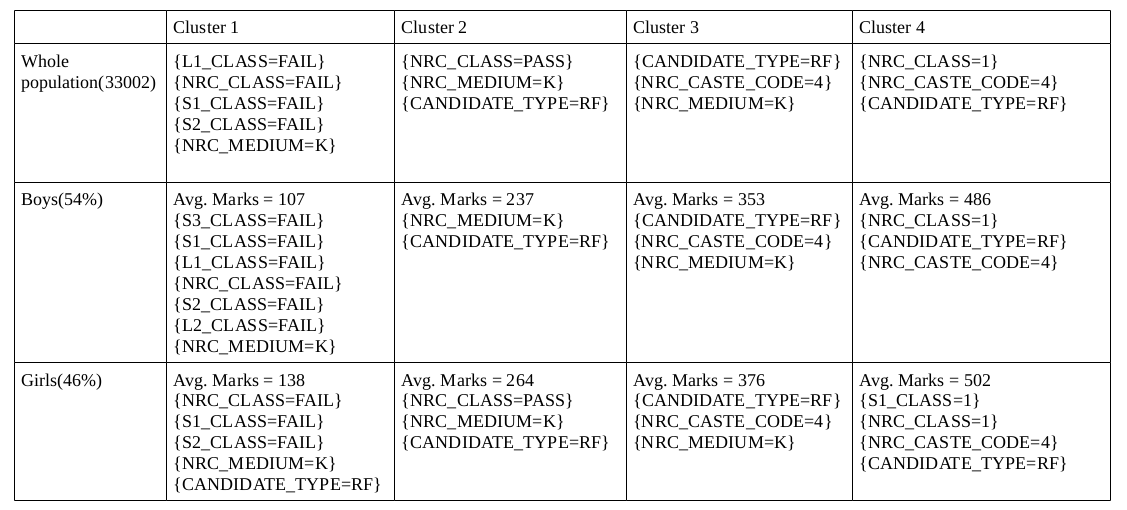
\includegraphics[scale=0.4]{img/boys_girls.png}

\item Partitioning based on URBAN{\_}RURAL

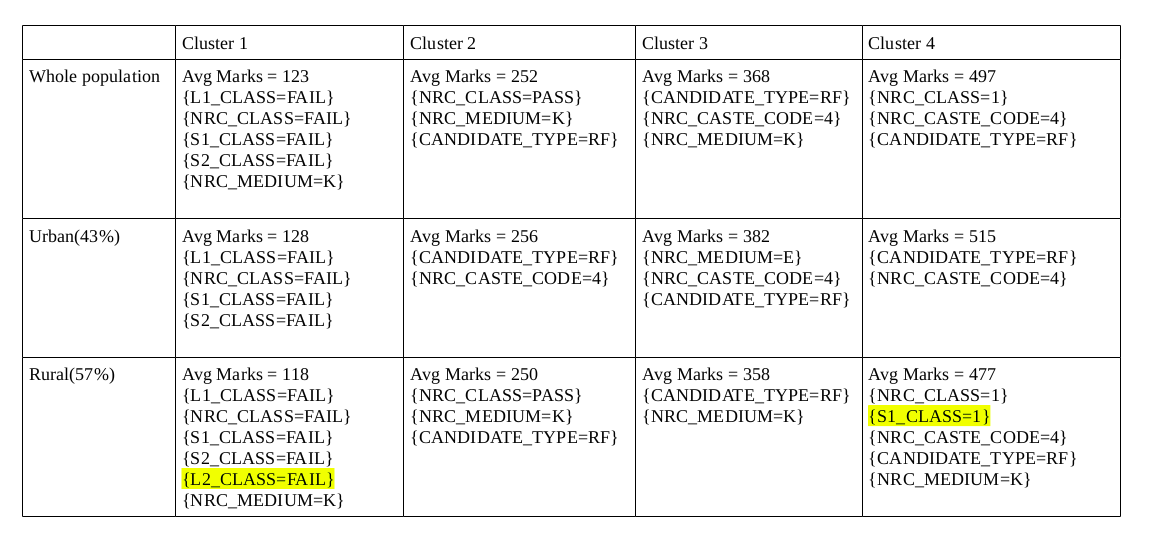
\includegraphics[scale=0.4]{img/urban_rural.png}

\end{itemize}


\section*{Conclusions}
\begin{itemize}
\item Partitioning based on URBAN{\_}RURAL

\begin{itemize}

\item Cluster 1 - Candidates who fail
\begin{itemize}
\item Urban - Their medium is not necessarily Kannada
\item Rural - They also fail in L2
\end{itemize}

\item Cluster 2 - Candidates who just pass
\begin{itemize}
\item Urban - Medium is not necessarily kannada and students belong to the general category.
\item Rural - Repeaters do not just pass. They either secure higher grades or fail(more likely).
\end{itemize}


\item Cluster 3 - Just missing First Class
\begin{itemize}
\item Urban - Medium is english.
\item Rural – Medium is kannada. Are not necessarily general category.
\end{itemize}



\item Cluster 3 - Just missing distinction
\begin{itemize}
\item Urban - There are a significant number of students who have gotten distinction.
\item Rural - Medium is kannada and have scored atleast 60 in mathematics.
\end{itemize}

\end{itemize}








\item Partitioning based on GENDER{\_}CODE

\begin{itemize}

\item Cluster 1 - Candidates who fail
\begin{itemize}
\item Boys - Fail in all subjects except L3, which is typically Hindi.
\item Girls - Do not fall in L1(Mostly Kannada). Most are regular freshers.
\end{itemize}

\item The other clusters have the same characteristics.

\end{itemize}


\end{itemize}
